\section{Задание}

Создайте HTML приложение. По нажатию на кнопку ``Показать'' приложение должно открыть новое окно и показать в нём портреты выбранного художника с короткими подписями.

\begin{center}
  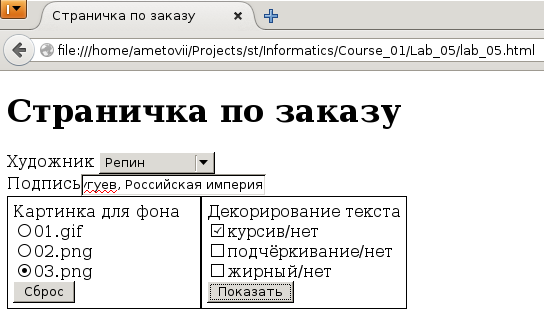
\includegraphics[width=10cm]{img/01.png}

  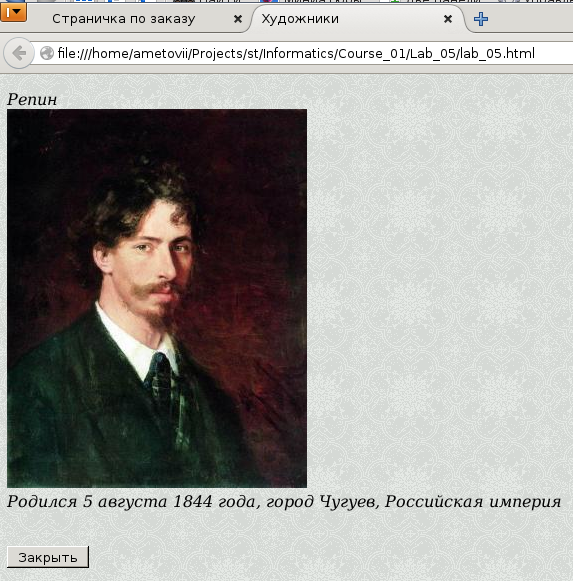
\includegraphics[width=10cm]{img/02.png}
  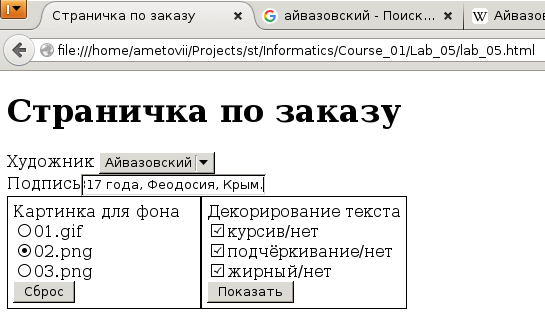
\includegraphics[width=10cm]{img/03.png}
  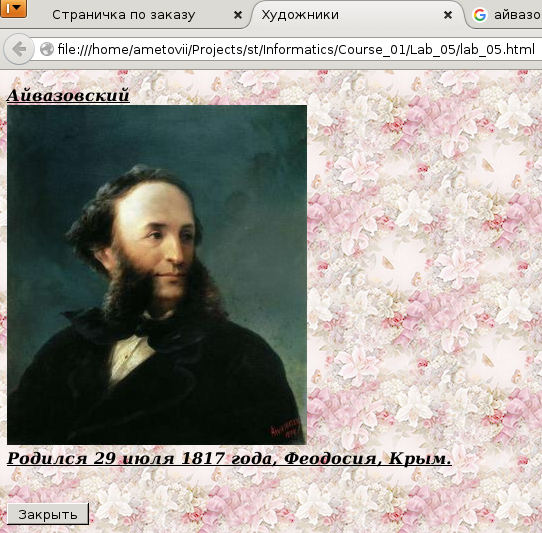
\includegraphics[width=10cm]{img/04.png}
\end{center}

Исходный код \verb|lab_05.html|:

\begin{verbatim}
<!doctype html>
<html>
  <head>
    <title>Страничка по заказу</title>
    <meta charset='utf-8' />
     <style type="text/css">
   .block1 { 
    padding: 5px;
    padding-right: 20px; 
    border: solid 1px black; 
    float: left;
   }
   .block2 { 
    padding: 5px; 
    border: solid 1px black; 
    float: left; 
   }
     </style>
     <script>
       function reset(){
	   document.getElementById('Ayvazovskiy').selected=true;
	   document.getElementById('someText').value="";
	   document.getElementById('k1').checked=true;
	   document.getElementById('c1').checked=false;
	   document.getElementById('c2').checked=false;
	   document.getElementById('c3').checked=false;
       }

       function go(){
	   var win=window.open();
	   win.document.open();
	   win.document.write(makeHeader());
	   win.document.write(addPainter());
	   win.document.write(makeFooter());
	   win.document.close();
       }

       function makeHeader(){
	   var backPicture1=document.getElementById('k1');
	   var backPicture2=document.getElementById('k2');
	   var backPicture3=document.getElementById('k3');
	   var str="<!DOCTYPE html><html><head><meta charset=\"ut"+
	   	 "f-8\"><title>Художники</title><style>body {back"+
		 "ground-image: url(";
	     if (backPicture1.checked) str=str+"Background/01.gif";
	     if (backPicture2.checked) str=str+"Background/02.png";
	     if (backPicture3.checked) str=str+"Background/03.png";
	     str=str+");}p{"
	     var boldText=document.getElementById('c3');
	     var italicText=document.getElementById('c1');
	     var underlineText=document.getElementById('c2');
	     if (boldText.checked) str=str+"font-weight: bold;";
	     if (italicText.checked) str=str+"font-style: italic;";
	     	 if (underlineText.checked) str=str+"text-decoration"+
		 ": underline;";
	   str=str+"}</style></head><body>";
	   return str;
       }

       function makeFooter(){
	   return "</body>";
       }

       function addPainter(){
	   var Ayvazovskiy=document.getElementById('Ayvazovskiy');
	   var Tropinin=document.getElementById('Tropinin');
	   var Repin=document.getElementById('Repin');
	   var someText=document.getElementById('someText');
	   var str="<p>";
	   if (Ayvazovskiy.selected) str=str+"Айвазовский<br><img "+
	       "src=\"Portraits/01.jpg\"/>";
	   if (Tropinin.selected) str=str+"Тропинин<br><img src=\"P"+
	       "ortraits/03.jpg\"/>";
	   if (Repin.selected) str=str+"Репин<br><img src=\"Port"+
	       "raits/02.jpg\"/>";
	   str=str+"<br>"+someText.value+"</p><br><input type=\"bu"+
	       "tton\" value=\"Закрыть\" onClick=\"window.close();\">";
	   return str;
       }
     </script>
     </head>
    <body>
      <h1>Страничка по заказу</h1>
      Художник
      <select>
	<option id='Ayvazovskiy'>Айвазовский</option>
	<option id='Tropinin'>Тропинин</option>
	<option id='Repin'>Репин</option>
      </select><br>
	Подпись<input id='someText'></br>
      <div class="block1">
	Картинка для фона<br>
      <input type='radio' id='k1' name='v' checked />01.gif<br>
      <input type='radio' id='k2' name='v' />02.png<br>
      <input type='radio' id='k3' name='v' />03.png<br>
      <input type='button' value="Сброс" onClick="reset()" />
      </div>
      <div class="block2">
	Декорирование текста<br>
	<input type='checkbox' id='c1' name='c1'>курсив/нет<br/>
	<input type='checkbox' id='c2' name='c2'>подчёркивание/нет<br/>
	<input type='checkbox' id='c3' name='c3'>жирный/нет<br/>
	<input type='button' value="Показать" onClick="go()"/>
      </div>
    </body>
</html>
\end{verbatim}
